\documentclass[11pt]{article}
\usepackage[utf8]{inputenc}
\usepackage[T1]{fontenc}
\usepackage{amsmath}
\usepackage{multicol}
\usepackage{geometry}
\usepackage{tikz}
\usetikzlibrary{shapes.geometric, 3d}
\usepackage{enumitem}
\usepackage{xcolor}
\usepackage{titlesec}

% Configurações de layout
\geometry{a4paper, left=1cm, right=1cm, top=0.5cm, bottom=1.2cm}
\setlength{\columnseprule}{0.4pt}
\setlength{\baselineskip}{1.0\baselineskip}

% Cores para títulos
\titleformat{\section}{\normalfont\Large\bfseries\color{blue}}{\thesection}{1em}{}
\titleformat{\subsection}{\normalfont\large\bfseries\color{red}}{\thesubsection}{1em}{}
\titleformat{\subsubsection}{\normalfont\normalsize\bfseries\color{black}}{\thesubsubsection}{1em}{}

\title{\textcolor{blue}{Poliedros: Características e Classificação}}
\author{Professor: Jefferson}
\date{}

\begin{document}

\maketitle
\vspace{-1cm}

\begin{center}
\large{Nome: \underline{\hspace{8cm}} \quad Turma: \underline{\hspace{3cm}}}
\end{center}

\begin{multicols}{2}

\section*{1. Conceito}
Um poliedro é um sólido geométrico tridimensional cujas faces são polígonos. Os elementos principais são:
\begin{itemize}
    \item \textbf{Faces}: superfícies planas poligonais
    \item \textbf{Arestas}: linhas onde duas faces se encontram
    \item \textbf{Vértices}: pontos onde arestas se encontram
\end{itemize}

\subsection*{Exemplos comuns}
\begin{itemize}
    \item Cubo
    \item Paralelepípedo
    \item Pirâmide
    \item Prisma
    \item Tetraedro
\end{itemize}

\section*{2. Relação de Euler}
Para poliedros convexos, vale a relação:
\[
V - A + F = 2
\]
onde:
\begin{itemize}
    \item $V$ = número de vértices
    \item $A$ = número de arestas
    \item $F$ = número de faces
\end{itemize}

\subsection*{Exemplo: Cubo}
\begin{itemize}
    \item $V = 8$ vértices
    \item $A = 12$ arestas
    \item $F = 6$ faces
    \item $8 - 12 + 6 = 2$ (confirma a relação)
\end{itemize}

\begin{center}
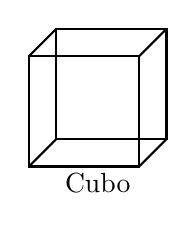
\begin{tikzpicture}[scale=0.7]
    \draw[thick] (0,0) -- (2,0) -- (2,2) -- (0,2) -- cycle;
    \draw[thick] (0.5,0.5) -- (2.5,0.5) -- (2.5,2.5) -- (0.5,2.5) -- cycle;
    \draw[thick] (0,0) -- (0.5,0.5);
    \draw[thick] (2,0) -- (2.5,0.5);
    \draw[thick] (2,2) -- (2.5,2.5);
    \draw[thick] (0,2) -- (0.5,2.5);
    \node at (1.25,-0.3) {Cubo};
\end{tikzpicture}
\end{center}

\section*{3. Classificação}
\subsection*{Poliedros de Platão}
São poliedros regulares onde:
\begin{itemize}
    \item Todas as faces são polígonos regulares iguais
    \item Todos os ângulos sólidos são iguais
    \item Existem apenas 5:
\end{itemize}

\begin{center}
\begin{tabular}{|l|c|c|c|}
\hline
Nome & Faces & Vértices & Arestas \\
\hline
Tetraedro & 4 triângulos & 4 & 6 \\
Cubo & 6 quadrados & 8 & 12 \\
Octaedro & 8 triângulos & 6 & 12 \\
Dodecaedro & 12 pentágonos & 20 & 30 \\
Icosaedro & 20 triângulos & 12 & 30 \\
\hline
\end{tabular}
\end{center}

\subsection*{Poliedros de Arquimedes}
Poliedros semi-regulares com mais de um tipo de face regular.

\section*{4. Prismas e Pirâmides}
\subsection*{Prismas}
\begin{itemize}
    \item Duas bases paralelas congruentes
    \item Faces laterais são paralelogramos
    \item Classificação pela base: triangular, quadrangular, etc.
\end{itemize}

\subsection*{Pirâmides}
\begin{itemize}
    \item Uma base poligonal
    \item Faces laterais triangulares que se encontram no ápice
    \item Classificação pela base: triangular, quadrangular, etc.
\end{itemize}

\begin{center}
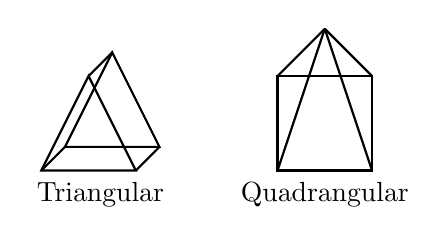
\begin{tikzpicture}[scale=0.6]
    % Prisma triangular
    \draw[thick] (0,0) -- (1,2) -- (2,0) -- cycle;
    \draw[thick] (0.5,0.5) -- (1.5,2.5) -- (2.5,0.5) -- cycle;
    \draw[thick] (0,0) -- (0.5,0.5);
    \draw[thick] (1,2) -- (1.5,2.5);
    \draw[thick] (2,0) -- (2.5,0.5);
    \node at (1.25,-0.5) {Triangular};
    
    % Pirâmide quadrangular
    \draw[thick] (5,0) -- (7,0) -- (7,2) -- (5,2) -- cycle;
    \draw[thick] (5,0) -- (6,3);
    \draw[thick] (7,0) -- (6,3);
    \draw[thick] (7,2) -- (6,3);
    \draw[thick] (5,2) -- (6,3);
    \node at (6,-0.5) {Quadrangular};
\end{tikzpicture}
\end{center}

\section*{5. Planificação}
Representação bidimensional de todas as faces do poliedro.

\subsection*{Planificação de um Cubo}
\begin{center}
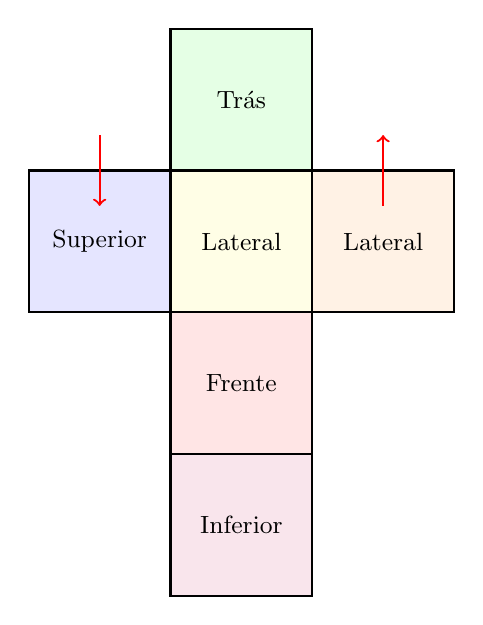
\begin{tikzpicture}[scale=0.9, every node/.style={font=\small}]
    % Faces principais (em forma de cruz)
    \draw[thick, fill=blue!10] (0,2) rectangle (2,4) node[pos=.5] {Superior};
    \draw[thick, fill=green!10] (2,4) rectangle (4,6) node[pos=.5] {Trás};
    \draw[thick, fill=red!10] (2,0) rectangle (4,2) node[pos=.5] {Frente};
    \draw[thick, fill=yellow!10] (2,2) rectangle (4,4) node[pos=.5] {Lateral};
    \draw[thick, fill=orange!10] (4,2) rectangle (6,4) node[pos=.5] {Lateral};
    \draw[thick, fill=purple!10] (2,-2) rectangle (4,0) node[pos=.5] {Inferior};
    
    % Linhas de dobra (tracejadas)
    \draw[dashed] (2,6) -- (2,-2);
    \draw[dashed] (4,6) -- (4,-2);
    \draw[dashed] (0,4) -- (6,4);
    \draw[dashed] (0,2) -- (6,2);
    
    % Setas indicando montagem
    \draw[->, red, thick] (1,4.5) -- (1,3.5);
    \draw[->, red, thick] (5,3.5) -- (5,4.5);
\end{tikzpicture}
\end{center}

\textbf{Observação:} As setas vermelhas indicam as direções para dobrar e montar o cubo.

\section*{6. Área e Volume}
\subsection*{Área Total}
Soma das áreas de todas as faces.

\subsection*{Volume}
Espaço ocupado pelo poliedro. Fórmulas comuns:
\begin{itemize}
    \item Cubo: $V = a^3$ (a $=$ aresta)
    \item Paralelepípedo: $V = abc$
    \item Prisma: $V = A_{\text{base}} \times h$
    \item Pirâmide: $V = \frac{1}{3} A_{\text{base}} \times h$
\end{itemize}

\section*{Exercícios Básicos (1-10)}
\begin{enumerate}
    \item Complete a tabela para os poliedros de Platão:
    \begin{center}
    \begin{tabular}{|l|c|c|c|}
    \hline
    Nome & Faces & Vértices & Arestas \\
    \hline
    Tetraedro & \hspace{1cm} & \hspace{1cm} & \hspace{1cm} \\
    Cubo & \hspace{1cm} & \hspace{1cm} & \hspace{1cm} \\
    Octaedro & \hspace{1cm} & \hspace{1cm} & \hspace{1cm} \\
    \hline
    \end{tabular}
    \end{center}
    
    \item Verifique a relação de Euler para um dodecaedro (12 faces pentagonais).
    
    \item Identifique os elementos:
    \begin{enumerate}[label=\alph*)]
        \item Número de arestas de um prisma hexagonal
        \item Número de vértices de uma pirâmide triangular
    \end{enumerate}
    
    \item Classifique os poliedros:
    \begin{enumerate}[label=\alph*)]
        \item Formado por 4 triângulos equiláteros
        \item Formado por 6 quadrados
    \end{enumerate}
    
    \item Desenhe a planificação de um tetraedro.
\end{enumerate}

\section*{Exercícios Avançados sobre Poliedros (11-30)}

\subsection*{Relação de Euler e Poliedros Convexos (11-20)}
\begin{enumerate}
    \item Um poliedro convexo tem 7 faces e 10 vértices. Quantas arestas possui?
    
    \item Determine o número de vértices de um poliedro com 12 faces triangulares e 30 arestas.
    
    \item Se um poliedro convexo tem 6 faces quadrangulares, qual é o número mínimo de vértices que ele pode ter?
    
    \item Um poliedro possui faces pentagonais e hexagonais, com 32 arestas. Sabendo que há 12 vértices, quantas faces pentagonais existem?
    
    \item Verifique a Relação de Euler para um icosaedro regular (20 faces triangulares, 12 vértices).
    
    \item Um poliedro convexo tem 3 faces quadrangulares e 4 triangulares. Calcule seu número de arestas.
    
    \item Determine o número de faces de um poliedro com 2 faces hexagonais e 12 triangulares, sabendo que possui 38 arestas.
    
    \item Se a soma do número de faces e vértices de um poliedro é 22, e ele tem 36 arestas, quantas faces possui?
    
    \item Um poliedro tem apenas faces triangulares e quadrangulares, com 18 arestas e 8 vértices. Quantas faces são quadrangulares?
    
    \item Desafio: Um poliedro convexo tem faces que são apenas pentágonos e hexágonos, com 3 arestas em cada vértice. Se possui 60 vértices, quantas faces pentagonais tem?
\end{enumerate}

\subsection*{Prismas e Pirâmides (21-24)}
\begin{enumerate}\setcounter{enumi}{20}
    \item Um prisma heptagonal regular tem \underline{\hspace{1cm}} faces, \underline{\hspace{1cm}} vértices e \underline{\hspace{1cm}} arestas.
    
    \item Uma pirâmide decagonal tem \underline{\hspace{1cm}} faces, \underline{\hspace{1cm}} vértices e \underline{\hspace{1cm}} arestas.
    
    \item Se um prisma tem 14 vértices, qual é o polígono de sua base?
    
    \item Determine o número de arestas laterais de uma pirâmide com base dodecagonal.
      
    
\end{enumerate}

\end{multicols}

\end{document}
